\documentclass{uwstat572}
\usepackage{amsfonts}
\usepackage{amssymb}
\usepackage{amsmath}
\usepackage{amsthm}
\usepackage{graphicx}
\usepackage{float}
\usepackage[caption = false]{subfig}
\usepackage[linesnumbered,algoruled,boxed,lined]{algorithm2e}

%%\setlength{\oddsidemargin}{0.25in}
%%\setlength{\textwidth}{6in}
%%\setlength{\topmargin}{0.5in}
%%\setlength{\textheight}{9in}

\usepackage{color}
\usepackage{ulem}
\newcommand{\vmdel}[1]{\sout{#1}}
\newcommand{\vmadd}[1]{\textbf{\color{red}{#1}}}
\newcommand{\vmcomment}[1]{({\color{blue}{VM's comment:}} \textbf{\color{blue}{#1}})}


\newtheorem{theorem}{Theorem}[section]
\newtheorem{proposition}{Proposition}[theorem]
\newtheorem{lemma}[theorem]{Lemma}

\theoremstyle{remark}
\newtheorem*{remark}{Remark}

\theoremstyle{definition}
\newtheorem{definition}{Definition}[section]

\SetKwInput{KwInit}{initialize}
\SetKwInput{KwJoin}{join}
\SetKwInput{KwSet}{set}

\renewcommand{\baselinestretch}{1.5} 


\bibliographystyle{plainnat}

\begin{document}
%%\maketitle

\begin{center}
  {\LARGE A Convex Formulation for Learning Scale-Free Networks via Submodular Relaxation}\\\ \\
  {Wayne Yang \\ 
    Department of Statistics, University of Washington Seattle, WA, 98195, USA
  }
\end{center}



\begin{abstract}
  To be completed.
\end{abstract}

\section{Introduction}
\citet{Defazio2012} present a novel method for estimating the structure of an undirected graphical model with a focus on Gaussian graphical models. In a graphical model, a random vector of dimension $p$ is represented by the graph $G = (V,E)$.  The vertices $v \in V$ represent each of the variables in the random vector and the edges $e \in E$ encode some form of association between two vertices. In the case of Gaussian graphical models, the edge set $E$ denotes the conditional independence structure of the variables.  Where the lack of an edge $e$ indicates the conditional independence of the two corresponding vertices given all of the other vertices.  As discussed in \cite{dempster}, the estimation of the structure of a Gaussian graphical model is equivalent to estimating the precision matrix.  The non-zero entries in the precision matrix signify the presence of an edge in the corresponding graph.  Therefore, determining the structure of a Gaussian graphical model boils down to a sparse estimate of the precision matrix.

The standard method for sparse estimation is currently an $l_1$ regularized maximum likelihood approach, introduced in \cite{Yuan2007}, which uses a Gaussian likelihood and a LASSO type penalty.  The estimator of the precision matrix, denoted $\widehat{\Theta}$, is defined to be
\begin{equation}\label{glasso}
    \widehat{\Theta} = \arg\min_{\Theta} -\log( \det( \Theta)) + tr(S \Theta) + \lambda \sum_{i, j} |\Theta_{i,j}|,
\end{equation}
where $S$ is the empirical covariance matrix and $\lambda$ is a non-negative tuning parameter. The diagonal terms $\Theta_{i,i}$ are sometimes excluded from the regularization term. The computation of this estimator or an approximate version of it is a well studied problem.  Examples include the neighborhood selection procedure from \cite{meinshausen2006}, block coordinate descent on the covariance matrix from \cite{Banerjee2008}, block coordinate descent on the precision matrix from \cite{Friedman2008}, alternating direction method of multipliers from \cite{Boyd2011}, and others.

While the standard $l_1$ method has been used successfully in many applications, it may perform poorly when the maximal degree of the latent graph $d$ is large relative to the dimension of the data $p$. Experimentally, \cite{Schaefer2005} construct graphs for which the standard method fails to identify hub vertices with large degrees. On the theoretical side, \cite{ravikumar2011} show that the minimum sample size for consistency of the $l_1$ regularized estimator in the $\| \cdot \|_{\infty}$ norm is of order $d^2 \log(p)$ which suggest that consistent estimation a precision matrix in a high-dimensional setting is difficult to achieve under the presence of hubs. Similar properties can be show for the neighborhood selection procedure in \cite{meinshausen2006}.  In the particular case of graphs with a degree distribution following a power-law (otherwise known as scale-free graphs), there are usually hub vertices that pose a problem for the standard method.  As a result, specialized techniques are required.

One existing method designed for scale-free graphs based on a reweighted $l_1$ regularization term was developed in \cite{liu11c}.  The Liu and Ihler method minimizes the objective
\begin{equation*}
    \widehat{\Theta} = \arg\min_{\Theta}  -\log( \det( \Theta)) + tr(S \Theta) + \alpha \sum_{i=1}^p \log( \| \Theta_{i,\neg}\|_1 + \varepsilon ) + \beta \sum_{i=1}^p |\Theta_{i,i}|,
\end{equation*}
where $\Theta_{i,\neg}$ denotes the $i^{th}$ row excluding the diagonal element.  The $\alpha$ and $\beta$ terms are non-negative tuning parameters and $\varepsilon$ is a positive offset to ensure the argument to log is not zero. While their experimental results are encouraging, the non-convexity of the objective induced by the log terms is undesirable because it complicates optimization and can only guarantee a local optimum.

The method proposed by \cite{Defazio2012} constructs an estimator which promotes a scale-free structure using a convex objective function motivated by viewing regularized likelihood estimation as Bayesian Maximum A Posteriori estimation.  The authors consider a prior placed on the edge set of the graph to obtain a combinatorial penalty based only on the degrees of the vertices. This combinatorial penalty is a submodular function on edge sets and admits a natural convex relation to Euclidean space to account for the real valued parameters required in a precision matrix. The resulting estimator is then the solution to a convex optimization problem. While the use of priors to promote scale-free structure was explored in \cite{sheridan2010}, the authors in that paper use MCMC to draw samples from the posterior distribution of the model parameters before computing an estimate.  \citet{Defazio2012}'s estimator can be efficiently computed as the exact solution to a convex program.

In this report, we will discuss the motivation, mathematical construction, and computation of the proposed method as well as evaluate the method's performance on both synthetic and real-world data.  We will also compare the method's performance against the standard $l_1$ procedure and the reweighted $l_1$ procedure.  

\section{Methods}

\subsection{Scale-Free Graphs}

There does not seem to be a consistent and precise definition of a scale-free graph across the literature (see \cite{li2005}).  However, most definitions share the requirement that the degree distribution of the graph be distributed according to a power-law. For our purposes, a graph is scale-free if 
\begin{equation}\label{powerlaw}
P(k) \propto k^{-r},
\end{equation}
where $P(k)$ is the proportion of vertices with $k$ neighbors and $r$ is a positive constant.  This particular definition was first used in \cite{Barabasi99} when describing the network topology of large networks in the real world.  However, empirical evidence of heavy tailed degree distributions was first observed in academic citation networks in \cite{de1965networks}.

One of the key features of scale-free graphs is the presence of hub nodes, or vertices with a large number of neighbors.  In some applications, correct identification of these hub nodes is a central concern.  For example, \cite{barabasi2004network} examines a number of biological networks, including protein-protein interaction networks and genetic regulatory networks, and notes that hub nodes may "fundamentally determine the network's behaviour."



\subsection{A Simplified Problem}

We first consider a simplified problem in which the values of the diagonal of the precision matrix are fixed and known and the off-diagonal entries are either zero or some known constant $\gamma$.  Under this simplification, we reduce the problem of covariance selection to finding which of the off-diagonal entries are non-zero.  As a result, a Bayesian estimation procedure needs only to assign a discrete prior distribution over possible edge sets of the underlying graph. To be precise, let $V$ be a set $p$ vertices corresponding to the dimension of the data.  For a given edge set $E$, we define a precision matrix $\Theta(E)$ with diagonal entries given by the fixed and known values and off-diagonal entries given by
\begin{equation*}
    \Theta(E)_{i,j} = \gamma {\bf{1}}_{\{(i,j) \in E\}}.
\end{equation*}
A posterior distribution can be formed by modeling the conditional distribution of the data $X$ to be a multivariate normal with mean zero and covariance matrix $\Theta(E)^{-1}$.  By concentrating prior probabilities on graphs that exhibit a scale-free structure, it is possible to encourage the final estimate to be scale-free.

Since the scale-free property is essentially a description of the degrees of the vertices in the graph, it is natural to construct a prior distribution that depends only on the degree profile.  To this end, the authors use an exponential random graph model parameterized by degree to form their prior.  For a fixed vertex set $V$, the probability distribution over edge sets $E$ is given by

\begin{equation}\label{cprior}
P( E ) \propto \exp \left( - \sum_{v \in V} h(d_E(v)) \right),
\end{equation}
where $d_E(v)$ denotes the degree of the vertex $v$ when the edge set of the graph is $E$ and $h \, : \, \mathbb{N} \to \mathbb{R}^+$ is a weighting function.  Particular choices $h$ will be discussed later.

Given the prior defined in equation \eqref{cprior}, the negative log of the posterior density of graph structure conditional on a sample $X_1,...,X_n$ is given by
\begin{equation}\label{logpost}
    -\log( P( E | X_1,...,X_n)) = - \log(L(\Theta(E) | X_1,...,X_n) ) + \sum_{v \in V} h( d_E(v)) + \text{constant},
\end{equation}
where $L$ denotes the likelihood function for a mean zero multivariate normal with covariance matrix $\Theta(E)^{-1}$. 

\subsection{Enforcing the Scale Free Property}

In order to concentrate the probability mass of this prior on scale-free graphs, the authors propose using $h(k) = \alpha \log(k + \varepsilon)$ for some positive constants $\alpha, \varepsilon > 0$.  Here, $\alpha$ is a  hyperparameter meant to reflect the scale of the power-law and $\varepsilon$ is an offset to ensure the argument to log is positive. In practice, $\alpha$ is a tuning parameter which controls the strength of the prior / regularization. While the authors do not formally prove that this probability distribution over edge sets satisfies any particular definition of scale-free, they do provide an informal motivation.  By plugging in this particular form of $h$ into equation \eqref{cprior}, the prior probability mass function becomes:
\begin{equation*}
    P( E) \propto \prod_{v \in V} (d_E(v) + \varepsilon)^{-\alpha}.
\end{equation*}
Note that if the degrees of the vertices $d_E(v)$ for $v \in V$ were mutually independent, then the marginal distribution of each $d_E(v)$ follows a power-law and samples from this distribution will tend to produce scale-free graphs.  However, independence does not hold because increasing the degree of one vertex necessarily increases the degree of some other vertex.  Unfortunately, it is not obvious how to assess the appropriateness of this heuristic motivation as the explicit computation of degree correlation is intractable.  Furthermore, our experiments indicate that choices of $h$ other than log provide superior results.

\subsection{Submodular Functions}

\theoremstyle{definition}
\begin{definition}
A set function $f \, : \, 2^E \to \mathbb{R}$ on $E$ is said to be a nondecreasing \text{submodular} function if for all $A \subseteq B \subseteq E$, the following two conditions hold:
\begin{equation*}
\begin{aligned}
1. \,& f(A) \leq f(B).
\\
2. \, & f(A \cup \{x\}) - f(A) \geq f(B \cup \{x\}) - f(B), \, \forall x \in E.
\end{aligned}
\end{equation*}
\end{definition}

The first condition ensure that we are dealing with a monotone set function. The second condition can be understood as a diminishing returns condition.  Adding any element $x$ to a smaller set yields a larger increase in $f$ than adding the same element to a larger set.

The reason that submodular functions are of interest in the context of this method is due to the form of the proposed prior.  Let $\mathcal{E}$ denote the set of of all possible edge sets for graph with a vertex set $V$.  For a given weighting function $h$, define a function $F \, : \, 2^{\mathcal{E}} \to \mathbb{R}$ by
\begin{equation}\label{F}
F(E) = \sum_{v \in V} h(d_E(v)).
\end{equation}
Note that in the expression for the  negative log posterior density for the simplified problem defined in equation \eqref{logpost}, the contribution of the prior is exactly $ F(E)$.  In the following lemma, we will show that with the appropriate choice of $h$, $F$ is in fact a submodular function.

\begin{lemma}
Let $h$ be a concave, non-decreasing function from $\mathbb{N} \to \mathbb{R}^+$, then $F$ as defined in equation \eqref{F} is a submodular function.
\end{lemma}
\begin{proof}
For a fixed vertex $v \in V$, we check that $d_E(v)$ is a submodular function on $\mathcal{E}$.  Fix any two subsets $A \subseteq B \subseteq \mathcal{E}$.  Trivially, $d_A(v) \leq d_B(v)$ since all edges connected to $v$ in $A$ are contained in $B$.  To check the submodularity condition, first observe that for any edge $e \in \mathcal{E}$ and any subset $C \subset \mathcal{E}$, we must have that $d_{C \cup \{e\}}(v) - d_{C}(v) \leq 1$.  Furthermore, for any $e$ not connected to $v$, then $d_{C \cup \{e\}}(v) - d_{C}(v) = 0$.  Finally, if $e$ is connected to $v$, then either $e \in A$ or $e \in A^C$.  If $e \in A$, then $A \cup \{e\} = A$ and $B \cup \{e\} = B$ which implies that the requirement of condition 2 is met.  On the other hand, if $e \in A^C$, then $d_{A \cup \{e\}} (v) - d_A(v) = 1$.  By the bound established earlier, the second condition holds in this case as well.  We conclude that
$d_E(v)$ is a submodular function.

It is shown in \cite{fujishige2005submodular} that a concave, non-decreasing transformation of a submodular function is submodular.  Thus, $h(d_E(v))$ is a submodular function.  Lastly, a non-negative linear combination of submodular functions is a submodular function.  We conclude that $F$ is submodular.
\end{proof}

For the remainder of the paper we will assume $h$ to be a concave, non-decreasing function.  We will also assume $h(0) = 0$ for convenience.  The fact that $F$ is submodular is important for two reasons.  The first is that generalizing beyond the simplified problem to regular covariance selection can be accomplished through a natural relaxation of $F$ via the Lov{\'a}sz extension.  This extension will be discussed more thoroughly in the next section.  The second reason is that the submodularity of $F$ places the authors' method in the context of a broader class of methods which induce structured sparsity through submodular functions as discussed in \cite{bach2010}. Submodular functions may offer a unified framework for developing new theory and methods aimed at problems leveraging a priori knowledge about the sparsity pattern in non-trivial ways.



\subsection{A Convex Relaxation}

While the discrete prior constructed for the simplified problem highlights the motivation for the main method in terms of the desired structure, the simplified problem does not apply to any real-world scenario.  In particular, the values of the entries in the precision matrix are almost always unknown parameters and assuming particular fixed values usually has no reasonable justification.  One possibility is to explicitly assign priors to the entries of the precision matrix and compute estimates via samples from the posterior as considered in \cite{sheridan2010}.  Alternatively, we can directly modify the form of the log posterior to accommodate unknown values of the precision matrix.  

Returning to equation \eqref{logpost}, we note that the likelihood term does not need to be modified as we can immediately allow for $\Theta$ to vary over all positive definite matrices.  On the other hand, the contribution of the prior $F$ is in terms of the edge set rather than the entries of precision matrix.  The authors propose relaxing $F$ from a set function to a function mapping $\mathbb{R}^{|\mathcal{E}|} \to \mathbb{R}$ by taking the convex envelope found using the Lov{\'a}sz extension, which is defined below.

\subsubsection{Definition}
Let $f \, : \, 2^E \to \mathbb{R}$ be a set function with $E = {1,...,N}$.  For a point $x \in [0,1]^N$ and $\lambda \in [0,1]$, define $T_{\lambda}(x) = \{i \in E \, : \, x_i \geq \lambda\}$.  Then the Lov{\'a}sz extension of $f$, denoted $\hat{f}$, is given by:
\begin{equation*}
\hat{f}(x) = \int_{0}^1 f( T_{\lambda}(x)) \, d\lambda.
\end{equation*}
More explicitly, take $x \in [0,1]^N$.  Let $x_{(1)} \geq \cdots \geq x_{(N)}$ be a reordering of the values of $x$.  Then, the $T_{\lambda}(x)$ is exactly:
\begin{equation*}
T_{\lambda}(x) = \begin{cases}
\{1,...,N\} & {\text{ if }} \lambda \in [0,x_{(N)}]
\\
\{1,...,i\} & {\text{ if }} \lambda \in (x_{(i+1)}, x_{(i)}]
\\
\varnothing & {\text{ otherwise}}.
\end{cases}
\end{equation*}
Therefore, the Lov{\'a}sz extension is exactly given by:
\begin{equation}\label{lovasz}
\begin{aligned}
\hat{f}(x) &= &&(1-x_{(1)}) f( \varnothing) + x_{(N)} f(\{1,...,N\})+ \sum_{i=1}^N f(\{1,...,i\})(x_{(i)} - x_{(i+1)}) 
\\
&= && f(\varnothing) + \sum_{i=1}^N (f(\{1,...,i\}) - f(\{1,...,i-1\})) x_{(i)}
\end{aligned}
\end{equation}
where $\{1,...,0\}$ corresponds to the empty set.

\begin{lemma}{Fextension}
The Lov{\'a}sz extension $\hat{F} \, : \, [0,1]^{|\mathcal{E}|} \to \mathbb{R}$ of the combinatorial penalty $F$ defined in \eqref{F} is given by
\begin{equation}
\hat{F}(x) = \sum_{i=1}^p \sum_{k=1}^{p-1} (h(k) - h(k-1)) x_{(i,k)},
\end{equation}
where each sequence $x_{(i,1)},...,x_{(i,p-1)}$ denotes the edges corresponding to the possible neighbors of $i$ in decreasing order.
\end{lemma}

\begin{proof}
We first consider the set function $F_v(E) = h(d_E(v))$ for a fixed vertex $v$. We extend $F_v$ to a map  $\hat{F}_v \, : \, [0,1]^{|\mathcal{E}|} \to \mathbb{R}$.  Notice that any edge $(i,j)$ where $i \neq v$ and $j \neq v$ is irrelevant to the evaluation of $F_v$. Therefore, the contribution of that edge to the sum in equation \eqref{lovasz} will be exactly zero. So without loss of generality, we need only consider the $p-1$ coordinates $x_{(v,i)}$ for $i \in V \setminus \{v\}$.  We also observe that $F_v( \{(v,1),...,(v,i)\}) = h(i)$ since $F_v$ depends only on the number of neighbors of $v$. Then the Lov{\'a}sz extension for $F_v$ is given by:
\begin{equation*}
    \hat{F}_v(x) = \sum_{i = 1}^{p-1} (h(i) - h(i-1)) x_{(v,i)}.
\end{equation*}
To compute $\hat{F}$, we sum the extensions $\hat{F}_v$ over all $v \in V$ since the Lov{\'a}sz extension of a sum of submodular function is the sum of their individual extensions.
\end{proof}


By Proposition 1 of \cite{bach2010}, we can obtain the convex envelope $\Omega$ of $F$ on $\mathbb{R}^{\mathcal{E}}$ to be the evaluation of the Lov{\'a}sz extension of $F$ on the absolute values of the entries of the off-diagonal elements of the precision matrix.  In other words, for each $i = 1,...,p$,  let $|\Theta_{i,(0)}| \geq \cdots \geq |\Theta_{i,(p-1)}|$ denote the off-diagonal elements of the $i^{th}$ row in decreasing order by absolute value.  Then, the convex envelope $\Omega$ is given by
\begin{equation}\label{omega}
\Omega(\Theta) = \sum_{i=1}^p \sum_{k=1}^{p-1} (h(k) - h(k-1)) | \Theta_{i,(k)}|.
\end{equation}
Equation \eqref{omega} is a slight abuse of notation as $\Theta \in \mathbb{R}^{p \times p}$ while the cardinality of the set of possible edges is only $|\mathcal{E}| = \binom{p}{2}$.  If we consider the $\Omega$ to be a function of the off-diagonal entries of symmetric matrices that is invariant to changes on the diagonal, the abuse of notation is not very important as it's still clear that $\Omega$ is convex over the space of symmetric matrices.  However, in section 2.8, we will require that the $\Omega$ be convex over the space of all matrices $\mathbb{R}^{p \times p}$. Fortunately, the convexity of this penalty can be proved directly.  

The use of a convex envelope as an approximation to a combinatorial penalty is not a new idea.  For example, the $l_1$ norm can be viewed as the convex envelope of the cardinality function on the support of a vector.  From this perspective, the usual $l_1$ regularization term can be seen as the convex relaxation of a penalty which counts the non-zero entries of the solution.

\subsection{The Estimator}

Plugging the convex relaxation derived in the previous section into equation 5, we obtain the proposed estimator for learning a scale-free precison matrix with unknown entries.  As before, let $S$ denote the empirical covariance matrix obtained from an i.i.d. sample of $n$ multivariate Gaussians of dimension $p$.  Then, for a fixed $h$ and constant $\alpha > 0$, the estimator is defined to be
\begin{equation}\label{estimator}
\widehat{\Theta}_{submod} = \underset{\Theta = \Theta^T, \, \Theta \succ 0}{\arg \min} - \log(\det(\Theta)) + tr(S \Theta) + \alpha \Omega(\Theta).
\end{equation}
Here, $\alpha > 0$ is a tuning parameter set by the user to control the strength of the regularization.  

The objective function for the estimator is strictly convex because $- \log \det(\Theta)$ is strictly convex, $tr(S \Theta)$ is linear, and $\Omega(\Theta)$ is convex in $\Theta$.  Therefore, if a minimum exists, then it must be unique.  Furthermore, we can apply the argument of Lemma 3 from \cite{ravikumar2011} to ensure a positive definite solution exists.  Note that $- \log \det \Theta$ is infinite for positive-semidefinite matrices, so the minimizer must be strictly positive definite, if it exists.  By Proposition 1 of \cite{bach2010}, $\Omega$ is a norm on the off-diagonal entries of $\Theta$.  Therefore, the minimization problem of equation \eqref{estimator} has an equivalent constrained version by Langrangian duality given by
\begin{equation}
\underset{\Theta = \Theta^T, \, \Theta \succ 0, \, \Omega(\Theta) \leq C(\alpha)}{\arg \min} - \log(\det(\Theta)) + tr(S \Theta)
\end{equation}
for a value $C(\alpha) > 0$ depending only on $\alpha$. Therefore, the entries of the off-diagonal are bounded and we need only to ensure that the diagonal entries do not diverge to infinity (which would send $- \log \det (\Theta)$ to negative infinity.  By Hadamard's inequality for positive definite matrices, we have that $\log \det (\Theta) \leq \sum_{i=1}^p \log (\Theta_{ii})$.  Therefore, we have the bound
\begin{equation}\label{hadamard}
\sum_{i=1}^p \Theta_{ii} S_{ii} - \log \det (\Theta) \geq \sum_{i=1}^p\Theta_{ii} S_{ii} - \log (\Theta_{ii}).
\end{equation}
Since $S_{ii}$ corresponds to a diagonal entry, it will be positive except in degenerate cases not considered here.  It's easy to see the lower bound in equation \eqref{hadamard} tends to infinity as $\sum \Theta_{ii}^2$ grows towards infinity.  This implies that $\widehat{\Theta}_{submod}$ is a well defined estimator.

While the method is motivated by a Bayesian perspective and the use of scale-free priors, the actual procedure is not intended to be truly Bayesian.  Since we are not fixing the values of the diagonal entries of $\Theta$, we are implicitly taking an improper uniform prior.  However, the authors made several references to the desire for a normalizable prior, which is obviously impossible with an improper prior.  Instead, it may be more correct to view the final estimator as a frequentist regularized likelihood method motivated by Bayesian ideas.



\subsection{Choices of $h$}

Ideally, $h$ should be chosen such that the expected degree distribution of sample graphs from the prior should match the degree distribution of the desired graph structure.  In principle, this can accomplished for a given graph via maximum likelihood estimation.  While maximum likelihood estimation for exponential random graphs, one could use sampling techniques such as the MCMC method developed in \cite{snijders2002markov}.  

The authors also propose other possible choices for $h$ satisfying the requirement that $h$ is monotone increasing and concave.  For example, a slight modification to the choice of logarithm could be
\begin{equation*}
    h(k) = \log(k + 1) + \beta k
\end{equation*}
for some $\beta > 0$.  This will smooth the prior in the sense that all edges now receive a baseline penalty given by $\alpha \beta$ in addition to the penalty induced by the log term.

Another possibility suggested by the authors is to take
\begin{equation*}
    h(k) = \sqrt{k+1} - 1 + \beta k.
\end{equation*}
The square-root penalty diminishes slower than the $\log$ term.  Note that taking $h$ to be the identity recovers the graphical LASSO, so we can view using the square-root (or any other power function) to be an interpolation between the $\log$ method and the graphical LASSO.



\section{Optimization}

In order to compute the estimator, the authors propose using Alternating Direction Method of Multipliers (ADMM).  Introduced in \cite{Boyd2011}, ADMM combines dual decomposition and augmented Lagrangians in order to solve convex programs of the form:
\begin{equation*}
    \min_{x,y} f(x) + g(y) {\text{  subject to }} Ax + By = c
\end{equation*}
with variables $x \in \mathbb{R}^n, \, y \in \mathbb{R}^m$ and parameters $A \in \mathbb{R}^{n \times p}, B \in \mathbb{R}^{m \times p}$ and $c \in \mathbb{R}^p$.  The objective function must be the sum of two convex functions $f$ and $g$.  In particular, if a convex objective function $h$ which can be written as $h(x) = f(x) + g(x)$, then the unconstrained minimization problem given by
\begin{equation*}
\min_{x} h(x) = \min_{x} f(x) + g(x)
\end{equation*}
can be solved by applying ADMM to the constrained problem given by
\begin{align*}
& \min_{x,y} f(x) + g(y) 
\\
& {\text{ subject to }} x - y = 0.
\end{align*}
This particular form applies to a number of regularized $M$-estimators such as the regular LASSO or the graphical LASSO where both the objective and regularization term are convex.  

As noted above, both the likelihood function and the penalty derived from the submodular functions are convex and ADMM can be applied. Following the algorithm on page 15 of \cite{Boyd2011}, the authors use the scaled form of the ADMM algorithm.  Fix a step-size parameter $\rho > 0$.  Initialize $\Theta^{(0)} = I_{p\times p}$ and $U^{(0)} = 0_{p \times p}$.  Then, given the values $\Theta^{(l)}$ and $U^{(l)}$ from the previous step, the $(l+1)^{th}$ iteration of ADMM is given by

\begin{align}
\Phi^{(l+1)} & =  \arg\min_{\Phi} \, -\log(\det(\Phi)) + tr(S \Phi) + \frac{\rho}{2}\| \Phi - \Theta^{(l)} + U^{(l)}\|_2^2
\label{likprox}
\\
\Theta^{(l+1)} & = \arg \min_{\Theta} \, \alpha \Omega(\Theta) + \frac{\rho}{2} \| \Phi^{(l+1)} - \Theta + U^{(l)} \|_2^2
\label{omegaprox}
\\
U^{(l+1)} & = U^{(l)} + \Phi^{(l+1)} - \Theta^{(l+1)}.
\label{resid}
\end{align}
These steps are sequentially computed until a stopping criterion is met.  The authors use the stopping criterion that both $\|\Theta^{(l+1)} - \Phi^{(l+1)}\|_2 < \epsilon$ and $\|\Theta^{(l+1)} - \Theta^{(l)}\|_2 < \epsilon$ for some small tolerance $\epsilon > 0$.  The first condition ensures that the equality constraint is satisfied and the second condition ensures that the solution is stable.  Note that the first $\Phi$ and $\Theta$ updates are both proximal operators.

The solution to the $\Phi^{(l+1)}$ update has a closed form solution as derived in \cite{Boyd2011} which is guaranteed to be positive definite even if $\Theta^{(l)} - U^{(l)}$ is not positive definite.  Take the eigenvalue-decomposition $\rho(\Theta^{(l)} - U^{(l)}) + S =  Q \Lambda Q^T$ with eigenvalues $\lambda_1,...,\lambda_p$.  For each $i = 1,...,p$, define $\lambda^{\prime}_i = \frac{\lambda_i + \sqrt{\lambda_i^2 + 4\rho}}{2 \rho}$.  Let $\Lambda^{\prime}$ be the $p \times p$ matrix with diagonal entries given by $\lambda^{\prime}_1,...,\lambda^{\prime}_p$ and off-diagonal entries set to zero.  Then the update to $X^{(l+1)}$ is exactly:
\begin{equation*}
X^{(l+1)} = Q \Lambda^{\prime} Q^T.
\end{equation*}
This solution can be obtained by considering the first order sub-gradient equations.  Details can be found in in \cite{Boyd2011}.

The update to $\Theta^{(l+1)}$ is considerably more complicated as $\Omega$ is not differentiable and depends on the row-wise order statistics.  Furthermore, the symmetry constraint implies non-obvious interactions between the different rows.  For example, changing the value of $\Theta_{i,j}$ may impact the rank of entries in rows $i$ and $j$. The authors use a dual decomposition method to compute the solution.  


\subsection{Proximal Operator of $\Omega$}

The dual decomposition method proposed by the authors solves the proximal operator defined in equation \eqref{omegaprox} by minimizing the objective over the space of all matrices with a symmetry constraint.  In other words, they solve the optimization problem defined by
\begin{equation}\label{dualdecomp}
\min_{\Theta \in \mathbb{R}^{p \times p}, \, \Theta = \Theta^T} \, \alpha \Omega(\Theta) + \frac{\rho}{2} \| \Phi^{(l+1)} - \Theta + U^{(l)} \|_2^2.
\end{equation}
The authors claim that this simply makes the existing symmetry constraint and making it explicit.  However, if is unclear whether or not the symmetry constraint alone guarantees a positive definite solution.  The solution would be guaranteed to be positive definite if the $\Phi^{(l+1)} + U^{(l)}$ could be guaranteed to be diagonally dominant, but that may not be true in general.  In practice, the results seem to be positive definite.

Note that the problem defined by \eqref{dualdecomp} is a strictly convex function with a linear equality constraint.  By Slater's constraint qualification, the problem must satisfy strong duality.  In other words, minimizing the primal is equivalent to maximizing the dual.  Denoting $Z = \Phi^{(l+1)} + U^{(l)}$, the dual function $g$ is given by
\begin{equation}\label{dual}
g(V) = \min_{\Theta \in \mathbb{R}^{p \times p} } \frac{\alpha}{\rho} \Omega(\Theta) + \frac{1}{2} \| \Theta - Z \|_2^2 + \frac{1}{2}\sum_{i=1}^p V_{i,*}^T ( \Theta_{i,*} - \Theta_{*, i}^T),
\end{equation}
where $V_{i,*}, \Theta_{i,*}$ are the $i^{th}$ rows of their respective matrices and $\Theta_{*,i}$ is the $i^{th}$ column of $\Theta$.  In this formulation, we have taken $V$ to be a skew-symmetric matrix such that $V = - V^T$.  This notation allows us to rewrite the last term of the expression as
\begin{equation*}
\frac{1}{2}\sum_{i=1}^p V_{i,*}^T ( \Theta_{i,*} - \Theta_{*, i}^T) = \sum_{i=1}^p V_{i,*}^T \Theta_{i,*}.
\end{equation*}
By completing the square, we can rewrite the minimizer $\Theta(V)$ of \eqref{dual} to be
\begin{equation*}
\begin{aligned}
\Theta(V) &= && \underset{\Theta \in \mathbb{R}^{p \times p}}{\arg\min} \, \frac{\alpha}{\rho} \Omega(\Theta) + \frac{1}{2} \| \Theta - Z \|_2^2 + \sum_{i=1}^p V_{i,*}^T \Theta_{i,*} + {\text{ const}}
\\
&= &&  \underset{\Theta \in \mathbb{R}^{p \times p}}{\arg\min} \sum_{i=1}^p \frac{\alpha}{\rho} \sum_{k=1}^{p-1} (h(k) - h(k-1)) |\Theta_{i,(k)}| + \frac{1}{2} \| \Theta_{i,*} - Z_{i,*} + V_{i,*} \|_2^2 + {\text{ const}},
\end{aligned}
\end{equation*}
where the constant does not depend on $\Theta$ or $V$.  Since the dual is defined as the minimum over all $\Theta \in \mathbb{R}^p$, we can evaluate the dual by solving the subproblems
\begin{equation}\label{subprobfull}
    \min_{\Theta_{i,*} \in \mathbb{R}^p} \frac{\alpha}{\rho} \sum_{k=1}^{p-1} (h(k) - h(k-1))|\Theta_{i,(k)}| + \frac{1}{2} \| \Theta_{i,*} - Z_{i,*} + V_{i,*} \|_2^2
\end{equation}
independently for each $i=1,...,p$.  In particular, we use this method to find $\Theta(V)$.

We observe that each subproblem defined by \eqref{subprobfull} is the sum of a convex function and a quadratic term.  This implies that there is a unique minimizer $\Theta^{\star}$ that defines the dual.  As a result, the subdifferential of $g$ contains only a single point and we conclude the dual is the differentiable with gradient given by:
\begin{equation*}\label{dualgrad}
\nabla g(V) = \Theta_{\star} - \Theta_{\star}^T.
\end{equation*}
With the gradient in hand, we are now ready to provide the algorithm for computing the proximal operator.

\begin{algorithm}[!htp]
  \KwIn{matrix $Z$, constants $\alpha$, $\rho$, tolerance $\epsilon$, step-size $\eta \in (0,1)$}
  \KwInit{$X = Z$, $V = 0_{p \times p}$}
  \Repeat{$\|X - X^T\| < \epsilon$}{
    \For{$l = 1,...,n$}{
        $w = \sigma(Z_{l,*} - V_{l,*})$ {\it \# $\sigma$ permutes the off-diagonal elements of a row into descending order by absolute value}
        \\
        $X_{l,\neg} = \sigma^{-1}(\text{{ solveSubproblem}}(w))$ 
        \\
        $X_{l,l} = Z_{l,l}$
    }
    $V = V + \eta(X - X^T)$
  }
  \Return{$X$}    
\caption{Dual Gradient Ascent}\label{alg1}
\end{algorithm}

The authors maximize the dual by gradient ascent and the explicit steps are given in algorithm \ref{alg1}.  The main difficulty is solving the subproblems. In algorithm 2, we describe the method used by the authors to solve the subproblems under the simplifying assumption of a pre-sorted input.  While similar to standard LASSO regression with an identity design matrix, the ordered penalty introduces complications.  Namely, when a block of consecutive order statistics in a particular row have the same absolute value, they behave as a single point with a penalty given by the average of their individual penalties.  In order to overcome this grouping, the authors use a disjoint-set data structure to keep track of the groups and their respective values. The proof of correctness is provided in the appendix.

\begin{algorithm}[!htp]
    \KwIn{vector $w \in \mathbb{R}^{p-1}$ with $|w_1| \geq \cdots \geq |w_{p-1}|$\}}
    \KwInit{disjoint-set data structure with set membership function $\gamma$}
    \KwInit{vectors $u = 0_{p-1}$, $x = 0_{p-1}$}
    \For{$k=1,...,n-1$}
    {
        $u_k = |w_k| - \frac{\alpha}{\rho} (h(k) - h(k-1))$
        \\
        $\gamma(k).value = u_k$
        \\
        $r = k$
        \While{$r > 1$ and $\gamma(r).value \geq \gamma(r-1).value$}
            {
                merge sets $\gamma(r)$ and $\gamma(r-1)$
                \\
                $\gamma(r).value = \frac{1}{|\gamma(r)|} \sum_{j \in \gamma(r)} u_j$
                \\
                $r = \min \gamma(r)$
        }
    }
        \For{$k=1,...,n$}
    {
        $x_k = {\text{sign}}(w_k) \cdot \max\{\gamma(k).value,0\}$
    }
    \Return{$x$}
    \caption{solveSubproblem}\label{alg2}
\end{algorithm}

The solution of the subproblem has been independently studied by \cite{su2016} in the context of variable selection for regression via an ordered LASSO penalty.  \cite{su2016} uses a slightly different stack-based algorithm to compute the solution and point out its connection to isotonic regression.


\section{Results}

In this section, we compare the performance of the submodular relaxation method against the reweighted $l_1$ method of \cite{liu11c} and against the standard graphical LASSO.  In order to perform these comparisons using simulated data, we construct ROC curves in two ways.  The first method is to use what we believe to be the same method as the authors, which consists of fitting a single model for each simulated sample and thresholding the absolute values of the off-diagonal entries to produce an ROC curve.  The second method is to fit multiple models at different regularization strengths to obtain a false positive rate and true positive rate for each model.

We also apply the method to a real data set, available online at LINK.  Since there is no way to validate our findings on this dataset, we only consider the qualitative differences between the methods through visualizations of the estimated graphs. We also highlight the sensitivity to choices of hyper-parameters.

\subsection{Synthetic Data}

In order to generate synthetic data, we first sampled random graphs from various distributions.  Then, the true precision matrix $\Theta$ for a given graph was computed by $\Theta_{i,j} = -0.2$ whenever the $(i,j) \in E$ and zero otherwise.  The diagonal entries $\Theta_{i,i}$ were set to be $\Theta_{i,i} = 0.5 - \sum_{j \neq i} \Theta_{i,j}$ in order to make the precision matrix diagonally dominant.  Then, 500 samples are drawn from a  $\mathcal{N}(0,\Theta^{-1})$ multivariate normal distribution to form an empirical covariance matrix, which is then standardized into a correlation matrix.

For the ROC curves computed using the thresholding method, we sampled graphs using both the preferential attachment model as well as a method for constructing graphs for a given degree sequence.  Degree sequences are generated using a Pareto distribution. For each random graph process, we first sampled data once to tune the methods.   The methods are tuned to AUC using the ROC curve obtained by thresholding and the parameters were found using random-search.  Then, thirty more samples are drawn and ROC curves computed for each of them.  The average ROC curves are displayed in figure 1.

\begin{figure}
\subfloat[][Preferential Attachment Model]{
    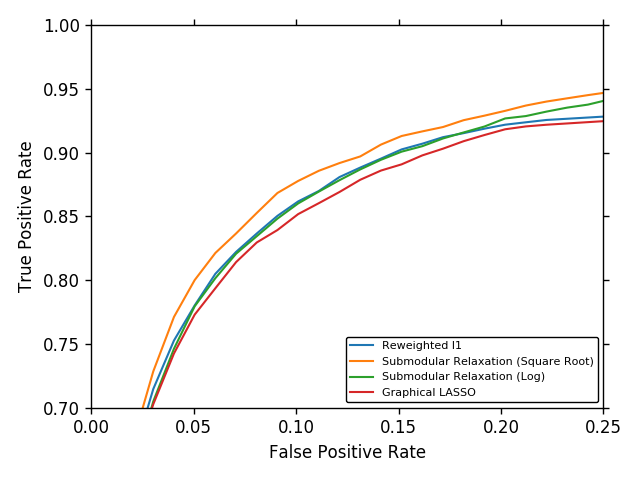
\includegraphics[width=0.5\linewidth]{PA-Threshold-ROC.png}
}
\subfloat[][Fixed Degree Sequence Model]{
    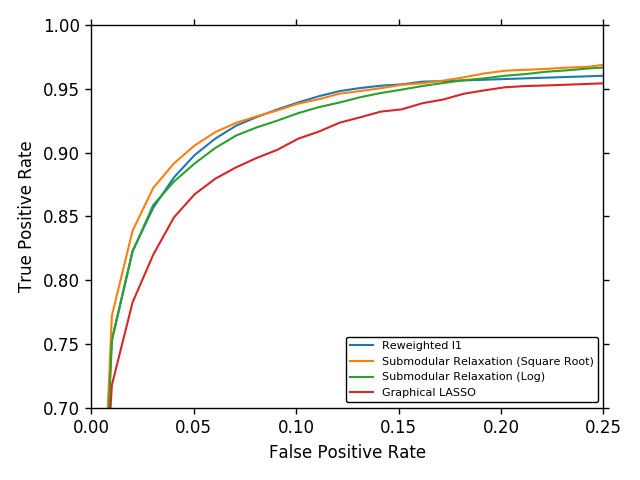
\includegraphics[width=0.5\linewidth]{bayatitestresults.png}
}
\caption{ROC curves obtained by thresholding estimates.}
\label{fig:threshold}
\end{figure}

While the submodular relaxation method with a square root weighting scheme appears to be superior to competing methods, there is a significant caveat to the perceived performance of the submodular relaxation method in figure 1.  Computing ROC curves in this particular way does not provide a good indication of the actual tradeoff between false positive rate (FPR) and true positive rate (TPR).  In particular, the goal of sparse estimation techniques is to produce a sparse parameter estimate without the use of post-hoc thresholding.  However, tuning to AUC will usually result choosing tuning parameters that produce dense estimates.  The actual FPR versus TPR trade-off should be understood as a function of the regularization strength.

However, this seems to match the ROC curves presented in \cite{Defazio2012}.  The authors also specifically note that the model is tuned on training data before the ROC curves are computed on test data.  In our attempts to reproduce these figures, tuning the method on other objectives such as accuracy or F1-score fails to produce dense graphs and thus the ROC curve cannot even be fully computed.  

For the ROC curves generated by varying the prior strength, we used three different graph structures including sample graphs from a preferential attachment model, sample Erdos-Renyi graphs, and a fixed star-shaped graph. For each sample, fifty different models are fit at different tuning parameter settings. For the submodular relaxation method, a small linear smoothing term is used but only the $\alpha$ parameter is changed.  The resulting FPR and TPR represent a single point on the ROC curve.  The full average ROC curves over thirty samples for each random graph process are shown in figure 2.  Particular portions of the same curves are displayed in figure 3. 

\begin{figure}
\centering
\subfloat[][Erdos-Renyi]{
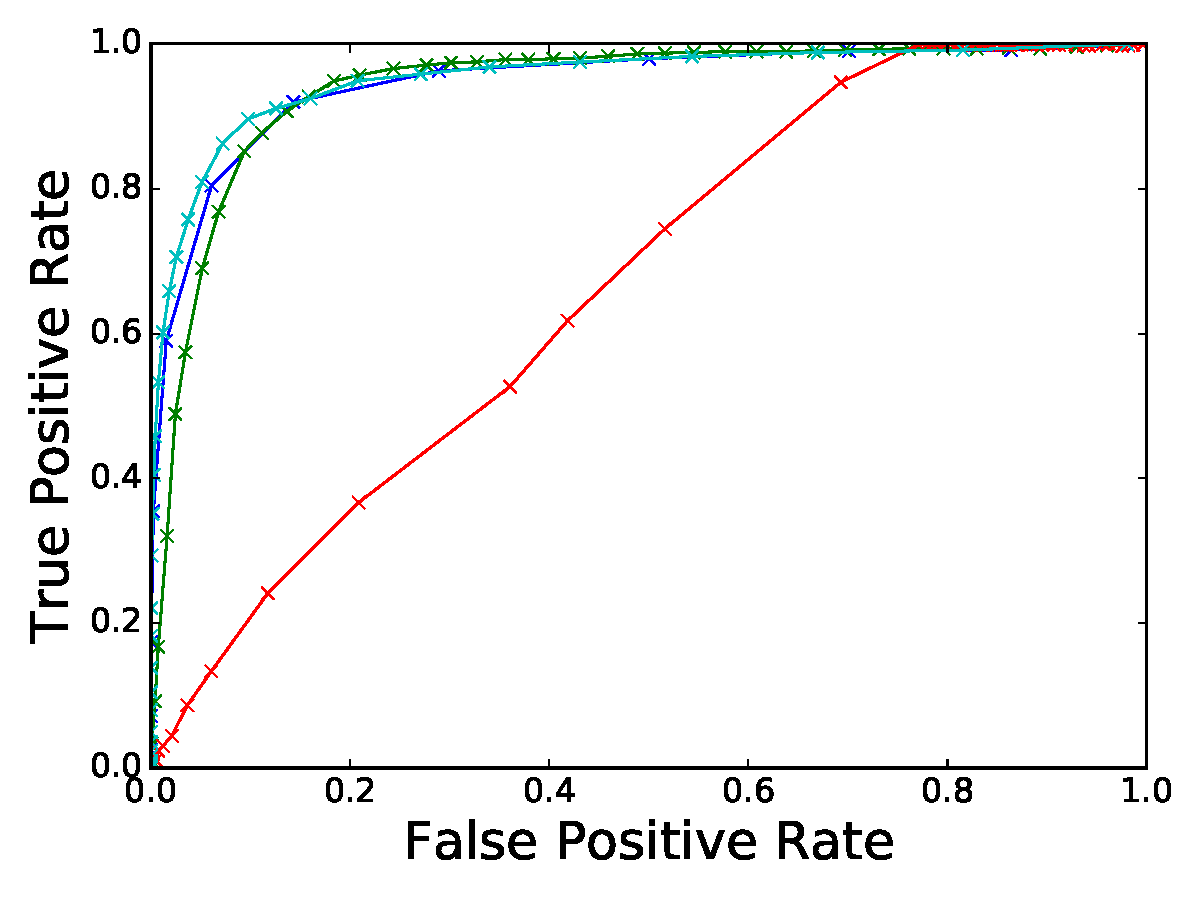
\includegraphics[width=0.5\linewidth]{ROC-params-erdos-full.pdf}
}
\subfloat[][Preferential Attachment]{
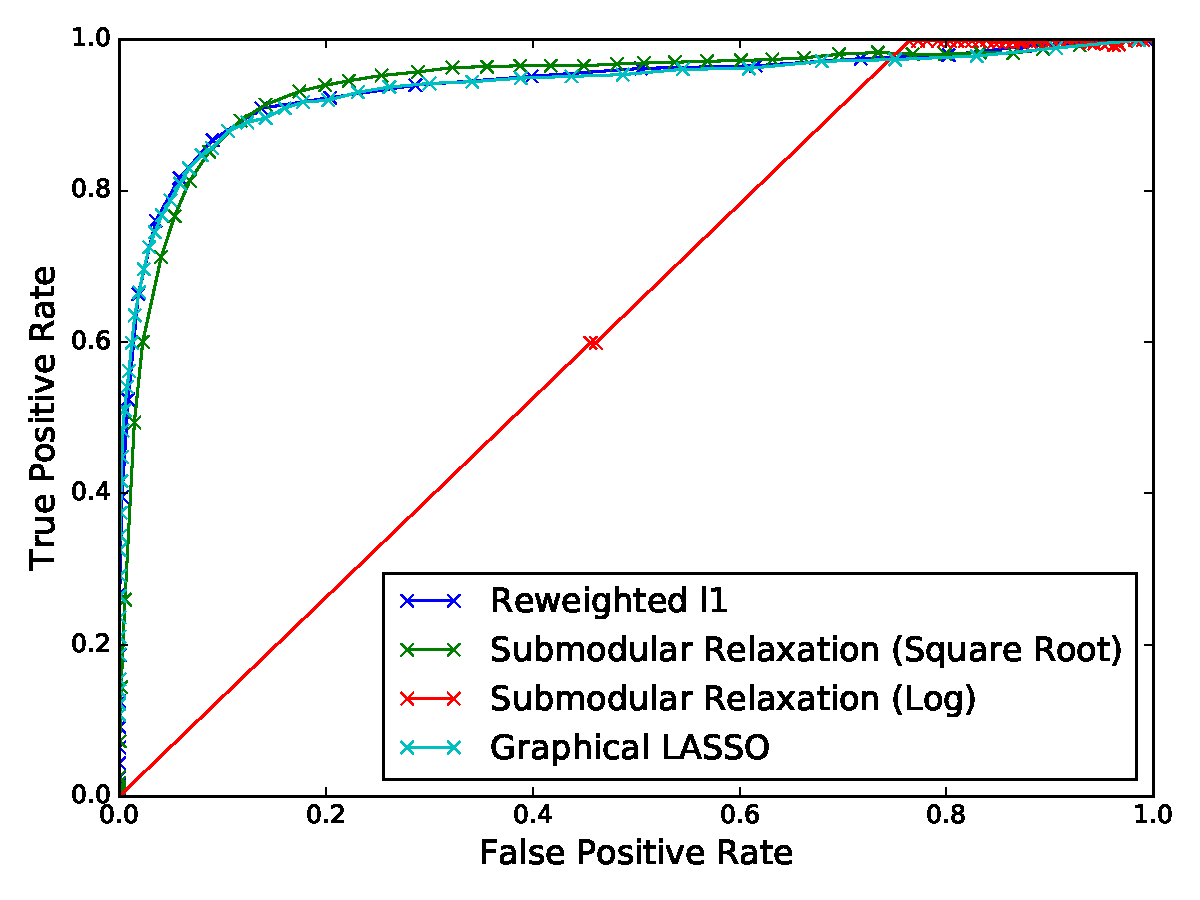
\includegraphics[width=0.5\linewidth]{ROC-params-PA-full.pdf}
}

\subfloat[][Star]{
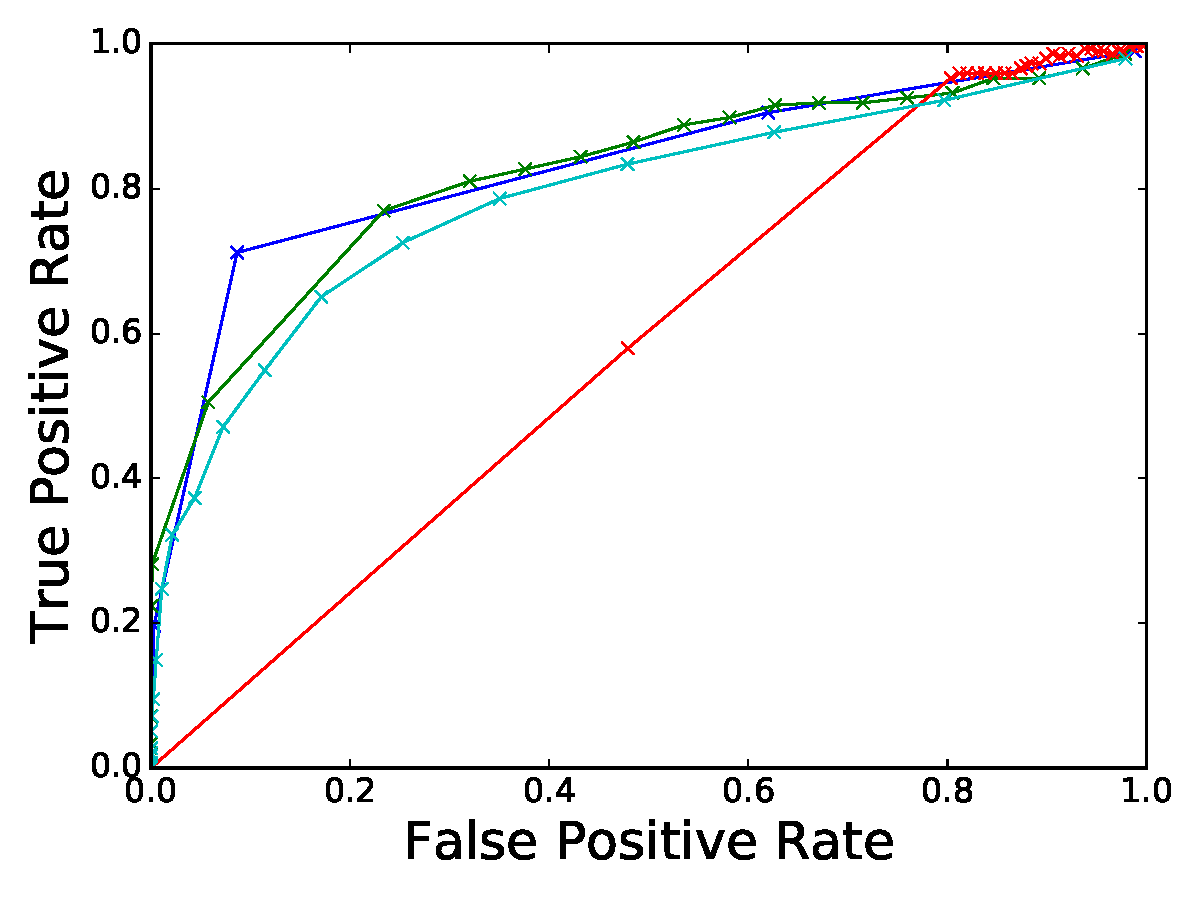
\includegraphics[width=0.5\linewidth]{ROC-params-Star-full.pdf}
}
\caption{ROC curves obtained by varying regularization for Erdos Renyi, Preferential Attachment, and star shaped graphs.}
\label{fig:paramfull}
\end{figure}

Before discussing the relative performance of the methods.  Note that the curves for the log based weighting scheme looks absurd in figure 2.  The concentration of points at high false positive rates indicates that there is a very sudden switch between producing dense precision matrices (which yield high false positive rates) and diagonal precision matrices.  While we do not have rigorous arguments to explain this phenomenon, we believe that this behavior is related to the decay of the penalty across the order statistics of a given row in the precision matrix.  In particular, the penalty associated with the smallest entry in a given row is orders of magnitude smaller than the penalty associated with the largest entry.  As a result, by the time the penalty is large enough for the lowest value to be driven to zero, the penalty on the larger entries may be many times larger.

\begin{figure}
\centering
\subfloat[][Erdos-Renyi]{
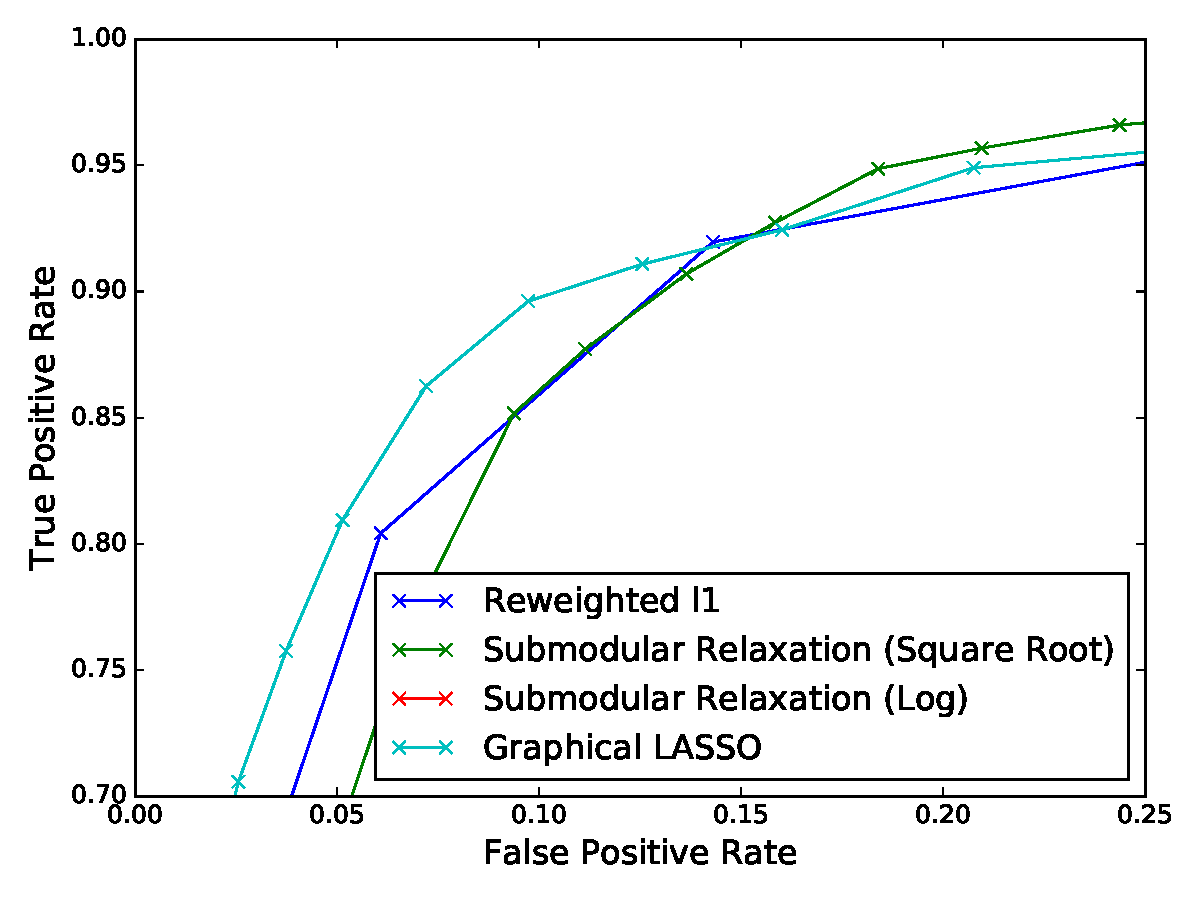
\includegraphics[width=0.5\linewidth]{ROC-params-erdos-part.pdf}
}
\subfloat[][Preferential Attachment]{
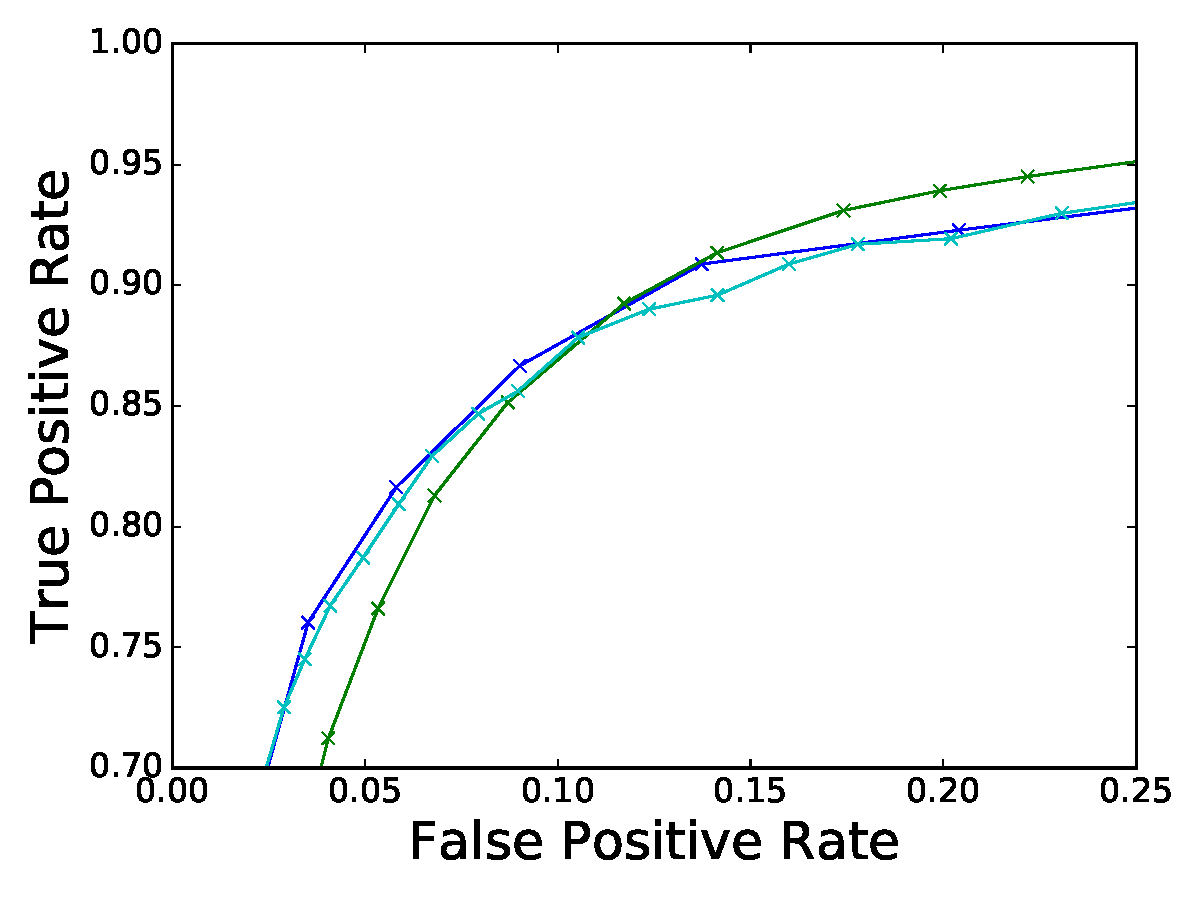
\includegraphics[width=0.5\linewidth]{ROC-params-PA-part.pdf}
}

\caption{ROC curves obtained by varying regularization for Erdos Renyi and Preferential Attachment graphs.}
\label{fig:parampart}
\end{figure}

Note that the curves for the preferential attachment model and the Erdos-Renyi model display similar patterns.  For lower false positive rates, the competing methods perform better on both.  However, there is a point on both curves at which the submodular relaxation begins to display better true positive rates.  Note that on the Erdos-Renyi curve, this change occurs at roughly fifteen percent false positive rate.  On the preferential attachment curve, this change occurs at roughly ten percent false positive rate.  In this sense, the submodular relaxation method does seem to perform better under the scale-free regime.  While we do not have formal arguments explaining this behavior, we believe that this is related to the decaying penalty.  The price of obtaining better accuracy for nodes with large degree seems to be the increase in spurious edges connected to nodes with low degree.  The tradeoff becomes more favorable as the graph size grows.  This is supported by the results for the star-shaped graph, where the methods aimed at scale-free graph structures are both superior to the graphical lasso.  





\subsection{Gene Expression Data}

The sample we used consists of 69 rats.  Expression levels were measured for 8565 genes using the rat liver cells.  We treat these vectors of expression levels as multivariate Gaussians.  Some missing values were found and were filled in with the value 1, which is what the authors used in their experiments.  Following \cite{Defazio2012}, we fit gene association networks on the first 500 genes using the submodular relaxation method, the graphical lasso, and the reweighted l1 methods by choosing tuning parameters which yield approximately 50 edges in the final estimate.  The choice of the first 500 is arbitrary and this data example serves only to illustrate the qualitative behavior of the estimators.  

The major connected component of each of the model fits and the degree distribution of that component is displayed in figure 4.  We note that both the submodular relaxation method and the reweighted $l_1$ method produce more pronounced hub vertices with many neighbors.  The degree distributions also reflect this behavior.  The submodular relaxation and the reweighted $l_1$ both produce degree distributions with heavier tails as one would hope when estimating a scale-free graph.

While the results of our experiments are encouraging, we were not able to reproduce the exact graphs presented in \cite{Defazio2012}, especially the star-shaped subgraph observed in their estimate obtained using the submodular relaxation method.  On the other hand, results obtained using the authors' publicly available implementation of the method agrees with our implementation.  

\begin{figure}
\centering
\subfloat[][Graphical Lasso]{
    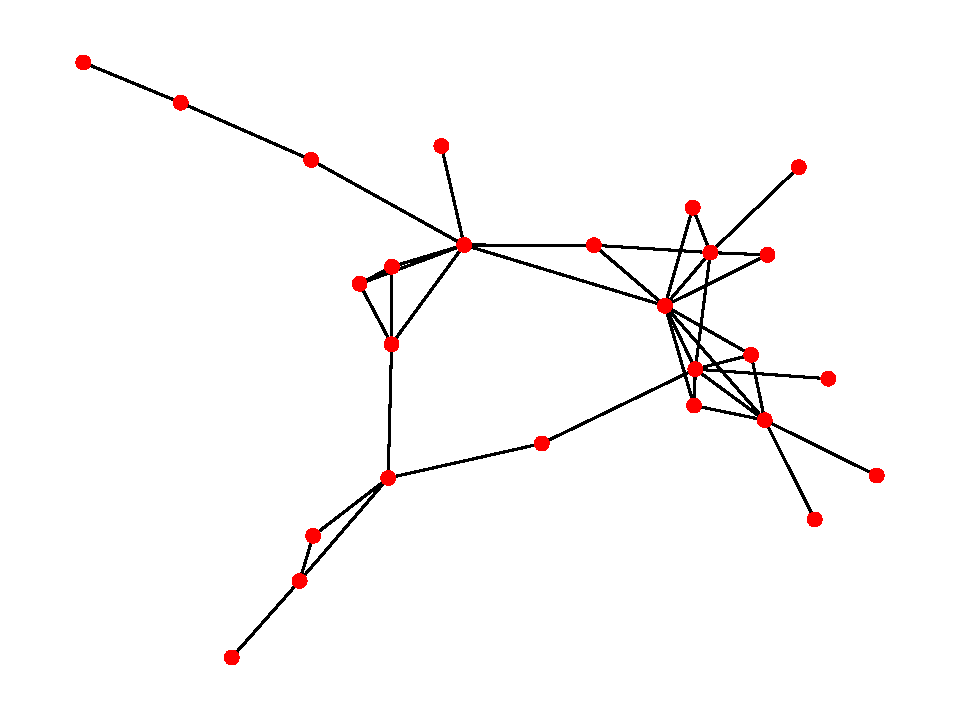
\includegraphics[width=0.3\linewidth]{glasso_graph.pdf}
}
\subfloat[][Submodular Relaxation]{
    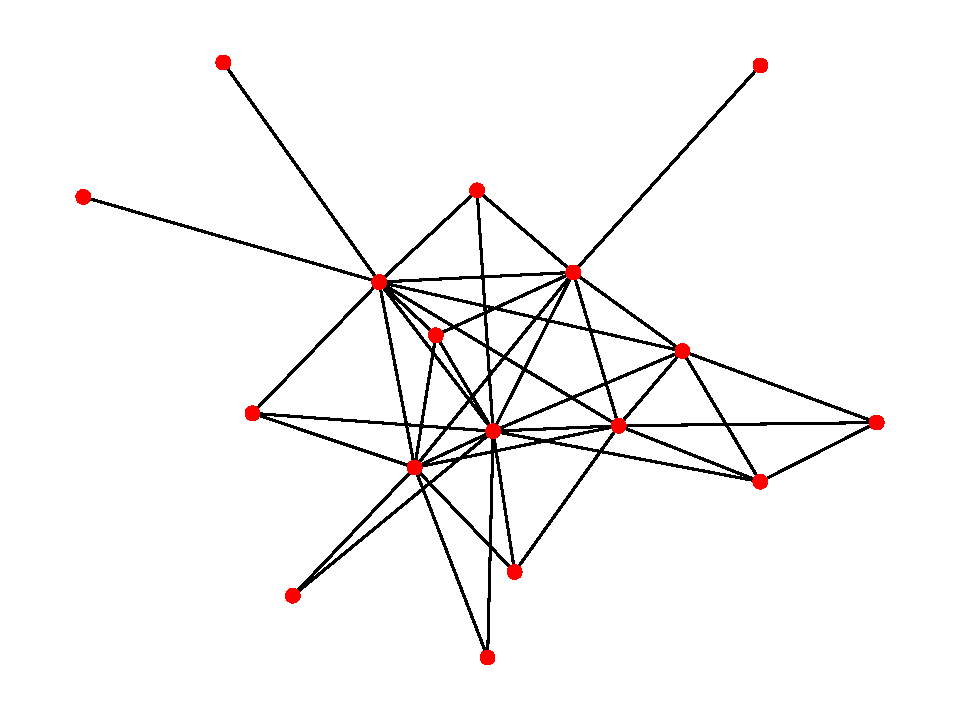
\includegraphics[width=0.3\linewidth]{submod_graph.pdf}
}

\centering
\subfloat[][Graphical Lasso]{
    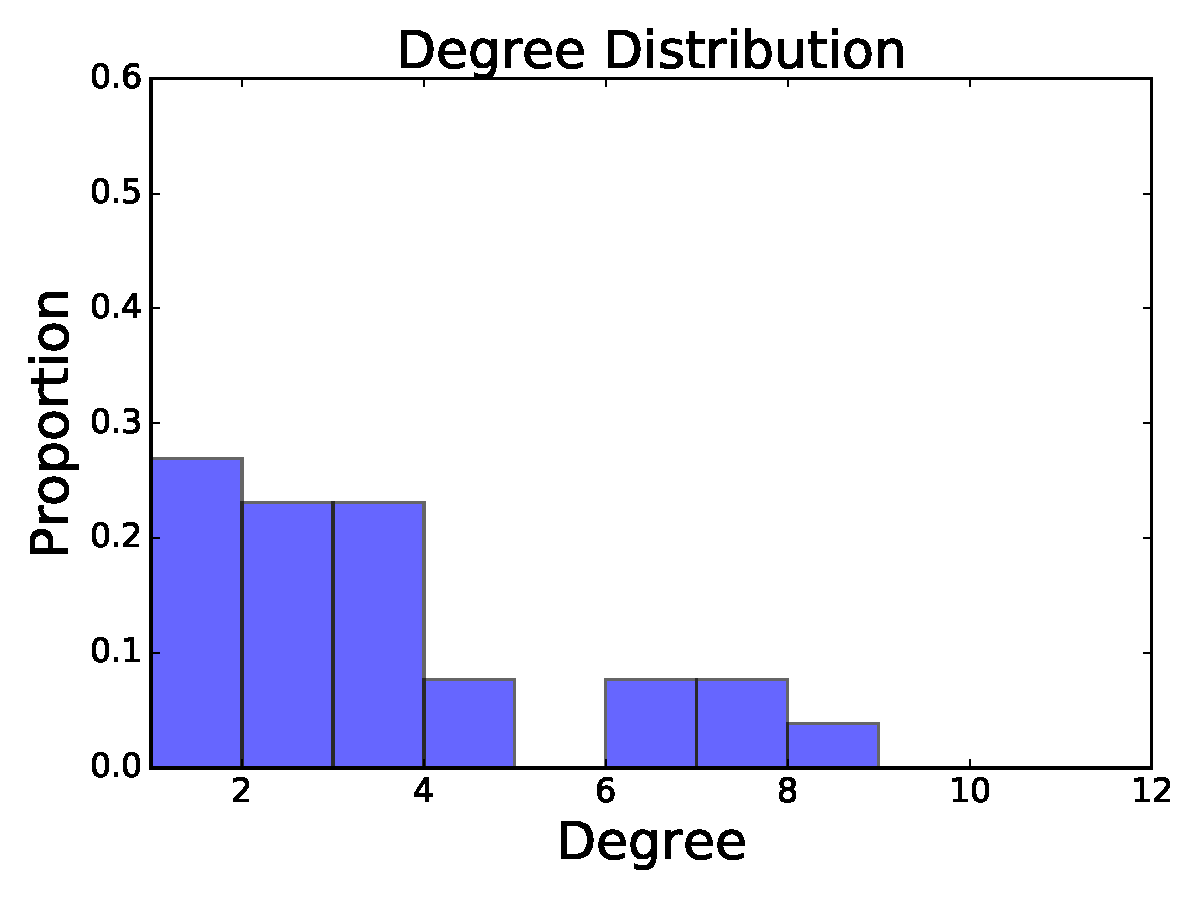
\includegraphics[width=0.3\linewidth]{glassodegree.pdf}
}
\subfloat[][Submodular Relaxation]{
    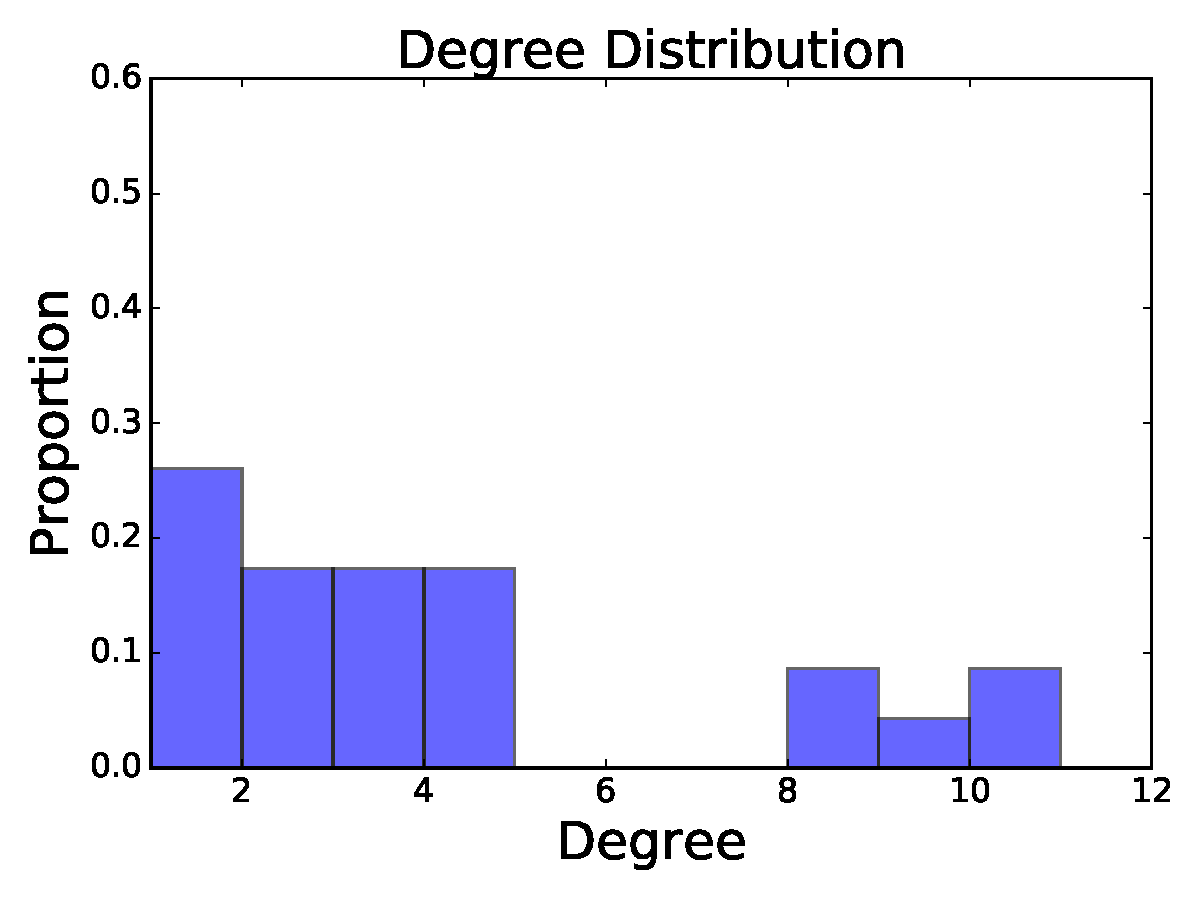
\includegraphics[width=0.3\linewidth]{submoddegree.pdf}
}


\caption{Largest connected components of estimated graph structures and their degree distributions.}
\label{graphs}
\end{figure}
We also observe that the tuning of the submodular relaxation method was extremely sensitive to the choice of tuning parameter.  In order to produce the graph displayed in figure 4, the linear smoothing term was chosen to dominate the square root portion of the penalty.  Recall that the penalty on $|\Theta_{i,(k)}|$ is given by
\begin{equation*}
    \alpha \left( h(k) - h(k-1) \right) = \alpha \left( \sqrt{k+1} - \sqrt{k} + \beta \right).
\end{equation*}
We took the $\beta = 0.8 \alpha^{-1}$ with $\alpha = 0.31$.  For comparison, we took the graphical LASSO tuning parameter $\lambda$, defined in \eqref{glasso}, to be $\lambda = 0.886$.  In other words, the submodular relaxation method was tuned so that it can be viewed as a slight modification to the graphical LASSO rather than an outright replacement.  

The sensitivity to the choice of tuning parameters also made it very difficult to fit a model by the usual cross-validation techniques or by Bayes Information Criterion.  In principle, one could fit models on a training subset and evaluate the likelihood of the hold-out validation set to choose the tuning parameters.  However, simple grid-search or random-search methods seem to produce poor results.  The optimal $\alpha$ changes dramatically when $\beta$ is changed.  On the other hand, for a fixed $\beta$, small perturbations to $\alpha$ lead to very different model fits. For instance, when tuning the model to produce around fifty edges for figure 4, taking $\beta = 0.7 \alpha^{-1}$ resulted in choosing an $\alpha$ value of $\alpha = 1.5$.  However, taking $\alpha = 1.7$ in that case led to an estimated graph with zero edges while taking $\alpha = 1.3$ yielded over 500 edges.  Ideally, tuning $\alpha$ and $\beta$ would involve selecting a number of $\beta$ values and then searching over a small region of $\alpha$ values for each $\beta$, but we were not able to come up with a sensible way to determine that region.


\section{Discussion}

\cite{Defazio2012} presents a method for estimating the latent structure of a graphical model when the underlying graph is believed to be scale-free.  The method is a regularized likelihood method with a convex penalty motivated by a Bayesian perspective on the estimation of graphical models and derived by submodular relaxation.  The convexity of the penalty makes it an attractive option when compared to non-convex alternatives for computational purposes and allows for global optimality guarantees when computing the estimator. Furthermore, our experiments suggest that the proposed penalty shows promise when handling graphs with hub vertices.  However, the observed sensitivity to tuning parameters means that further careful analysis and experiments are required before the method can be applied in actual data analysis settings.  In particular, a clear and principled approach to balancing the linear smoothing term and the decaying penalty in the choice of weighting function is central to the success of the method in a real-world setting.


\bibliography{stat572}

\end{document}









Understanding and estimating the structure of the edge set $E$ is an important task in fields such as social network analysis or bioinformatics.  For example, graphical models may be fit to gene expression data in order to estimate a gene expression network as described in  or to identify individual genes which have a large influence on the network.


Both the reweighted $l_1$ method and the convex relaxation method can both be thought of as part of a larger class of procedures which induce {\textit{structured}} sparsity in parameter estimates, where prior knowledge about the sparsity pattern can be exploited.  Examples include the group LASSO in \cite{Yuan06}, the fused LASSO in \cite{Tibshirani05sparsityand}, and trend filtering in \cite{Kim09trend} which all encode some desired properties in parameter estimates beyond simple sparsity.  Furthermore, the Defazio and Caetano is an example of the connection between submodular functions and sparsity inducing forms discussed in \cite{NIPS2010_3933}.


\subsection{Solution to the Subproblem}

For notational convenience, we will describe the algorithm for the problem defined by
\begin{equation}\label{subprobsimple}
\min_{x \in \mathbb{R}^p} \frac{1}{2} \|y - x\|^2 + \sum_{i=1}^p \lambda_{i} |x_{(i)}|
\end{equation}
with $\lambda_{1} \geq \cdots \geq \lambda_{(p)}$ and $|x_{(1)}| \geq \cdots \geq x_{(p)}|$.  We assume without loss of generality that $y_{1} \geq \cdots \geq y_{p} \geq 0$.  This is because the sign of each coordinate in the solution must match the sign of the corresponding coordinate of $y$.  Therefore, we can solve the problem for a non-negative vector $y$ and then reverse the signs later.  Since the penalty only depends on the order statistics, we can also apply a permutation to $y$ to put it in sorted order and then apply the inverse permutation to the solution later.  Furthermore, the following lemma from \cite{su2016} shows that the sort order of the solution matches the sort order of the target $y$.

\begin{lemma}\label{ordering}
When $y_1 \geq \cdots \geq y_p \geq 0$, the solution $x$ to \eqref{subprobsimple} satisfies $x_1 \geq \cdots \geq x_p \geq 0$.
\end{lemma}
\begin{proof}
Suppose by contradiction $x_i < x_j$ for $i < j$ with $y_i \geq y_j$.  The consider the vector $x^{\prime} = x$ except with $x^{\prime}_i = x_j$ and $x^{\prime}_j = x_i$.  Taking $f$ to be the objective function, we have that
\begin{equation*}
f(x) - f(x^{\prime}) = \frac{1}{2}(y_i - x_i)^2 + \frac{1}{2} (y_j - x_j)^2 - \frac{1}{2}(y_i - x_j)^2 - \frac{1}{2} (y_j - x_i)^2.
\end{equation*}
This follows from the fact that swapping $x_i$ and $x_j$ affects neither the regularization term nor the other quadratic terms.  A simple calculation gives
\begin{equation*}
    f(x) - f(x^{\prime}) = (x_j - x_i)(y_i - y_j) > 0,
\end{equation*}
which contradicts the optimality of $x$. 
\end{proof}
Lemma \ref{ordering} implies that we can reformulate \eqref{subprobsimple} as 
\begin{align}
& \min_{x} \frac{1}{2} \|y-x\|^2 + \sum_{i=1}^p \lambda_i x_i 
\\
& {\text{subject to }} x_1 \geq \cdots \geq x_p \geq 0.
\end{align}
Using this form of the problem, we can explicitly compute subgradients.  For $x_i$ not equal to any other $x_j$, the partial derivative is given by
\begin{equation*}
    \frac{\partial f}{\partial x_i}(x) = x_i - y_i + \lambda_i.
\end{equation*}
Which is similar to the 